% !TeX root = bachelorarbeit.tex
\label{num_pot}
\begin{Bemerkung}
	Die beiden folgenden Abschnitte bauen im Wesentlichen auf den beiden Vorlesungen 'Einführung in das Wissenschaftliche Rechnen' (SS 2019) und 'Finite Elemente Methoden' (WS 2019/2020) von Herrn Prof. Dr. Wieners auf. Dem entsprechend sind als Quellen neben \cite{brenner2007mathematical},
	\cite{braess2013finite} und \cite{hanke2002grundlagen} vor allem die Mitschriebe zu den oben genannten Vorlesungen, sowie die Berichte zum Rechnerpraktikum mit M++ \cite{siteM++} zu nennen.
\end{Bemerkung}
Wie bereits in obigem Abschnitt erwähnt, sollen sich die nächsten beiden Abschnitte damit beschäftigen, wie wir die oben beschriebenen Probleme für ein festes $\omega \in \Omega$ numerisch lösen können. 
Ein Überblick über alle möglichen Verfahren, welche zur Lösung der beiden Probleme geeignet sind, würde den Rahmen dieser Thesis sprengen. Wir wollen deshalb im Folgenden auf eine Möglichkeit eingehen diese Berechnung numerisch durchzuführen. Insbesondere werden dabei jene Verfahren beschrieben, welche wir auch später innerhalb der MLMC Methode in M++ nutzen wollen.
Da wir in diesen beiden Abschnitte $\omega \in \Omega$ ohnehin fest halten, genügt es zudem das deterministische Problem zu betrachten. \newline
Sowohl das hybride Finite Elemente Verfahren, welches wir zur Lösung des Potentialströmungsproblem nutzen wollen, als auch das Discontinuous Galerkin Vefahren, mit dessen Hilfe wir das Transportproblem lösen wollen, bauen auf der Finite Elemente Theorie auf. 
Diese ist im Wesentlichen in der zweiten Hälfte des 20. Jahrhunderts entstanden, ist aber bis heute in praktischer wie auch in theoretischer Sicht aktuell.
Die Grundidee ist hierbei die vorliegenden Rand-Anfangswertaufgaben in einem passenden endlichen Unterraum zu lösen. Dabei löst man sich auf analytischer Seite zunächst oft von einzelnen Regularitäts- und Differenzierbarkeitsbedingungen und führt einen sogenannten schwachen Lösungsbegriff ein (vergleiche Abschnitt 2.1). Statt nun aber solch eine schwache Lösung in einem unendlich dimensionalen Funktionenraum, wie beispielsweise in den Sobolevräumen $W^{1,2}(\mathbb{D})$ oder $W_0^{1,2}(\mathbb{D})$ zu bestimmen, zieht man sich auf endliche Unterräume zurück. \newline
Die folgende Definition entstammt \cite{brenner2007mathematical} und geht ursprünglich (1978) auf Ciarlet zurück.
\begin{Definition}\
	Sei
	\begin{itemize}
		\item $K \subseteq \R^d$ eine beschränkte abgeschlossene Menge mit einem nichtleeren Inneren und stückweise stetig differenzierbarem Rand 
		\item $\mathcal{P}$ ein endlich dimensionaler Funktionenraum auf K
		\item $\mathcal{N} = \{N_1,N_2,\dots,N_k \}$ eine Basis für $\mathcal{P}^{'}$
	\end{itemize}
	Dann heißt $(K,\mathcal{P},\mathcal{N})$ ein finites Element.
\end{Definition}

Wir wollen im Folgenden diese theoretische Definition zwar im Hinterkopf behalten, aber wie in \cite{braess2013finite} meist nur mit den sogenannten Finite-Elemente-Räumen arbeiten. 
Dabei wird eine geeignete Zerlegung $\mathfrak{K} = \{K_1,K_2,\dots, K_M \}$ von $\mathbb{D}$ in endlich viele Teilgebiete gewählt. 
Anschließend betrachten wir einen endlichen Raum von Funktionen, die eingeschränkt auf diese Teilgebiete von einfacher Gestalt sind, beispielsweise bieten sich oft polynomielle Darstellungen niedrigen Grades an. 
Ein solches Teilgebiet $K \in \mathfrak{K}$ nennen wir Finites Element oder auch Zelle und fordern implizit verbunden mit dem betrachteten Funktionenraum die Erfüllung der obigen Definition. \newline
Im Falle $\mathbb{D} \subseteq \R^2$ kommen so z.B. Dreiecke oder Vierecke in Frage, in $\mathbb{D} \subseteq \R^3$ können Tetraeder, Würfel, Quader und andere genutzt werden. \newline
Sei nun $\mathbb{D} \subseteq \R ^2$ zudem ein polygonales Gebiet, um eine einfache Zerlegung in Dreiecke oder Vierecke zu gewährleisten.

\begin{Definition}
	\begin{enumerate}
		\item Eine Zerlegung $\mathfrak{K} = \{ K_1,K_2,\dots,K_M\}$ von $\mathbb{D}$ in Dreiecks- oder Viereckselemente heißt zulässig, wenn folgende Eigenschaften erfüllt sind:
		\begin{itemize}
			\item $\overline{\mathbb{D}} = \bigcup_{i=1}^M K_i$
			\item Für $i \neq j$ ist $K_i\cap K_j$
			\begin{enumerate}
				\item ein gemeinsamer Eckpunkt von $K_i$ und $K_j$
				\item eine gemeinsame Kante von $K_i$ als auch von $K_j$
				\item oder $K_i\cap K_j= \emptyset$
			\end{enumerate}
			
		\end{itemize}
		\item Wir schreiben oft $\mathfrak{K}_h$ anstatt $\mathfrak{K}$, wenn jedes Element einen Durchmesser von höchstens $2h$ besitzt [Vorlesung h = max diam K was passt besser]
	\end{enumerate}
\end{Definition}

\begin{figure}[H]
	\centering
	\captionabove{Zulässige Zerlegung und unzulässige Zerlegung mit hängendem Knoten}
	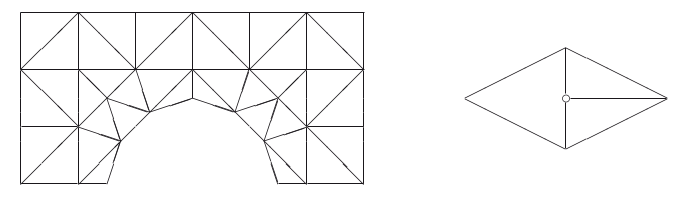
\includegraphics[width=0.8\textwidth]{triangulierung.png} \\
	Abbildung aus \cite{braess2013finite} Seite 58
\end{figure}
Wir führen außerdem folgende Bezeichnungen ein:
\begin{itemize}
	\item ein $ K \in \mathfrak{K} $ nennen wir Zelle
	\item $ \mathbb{D}_h \coloneqq \bigcup_{K \in \mathfrak{K}} K $ sei die Menge der Zellen
	\item ein $ z \in \mathcal{V}_K \coloneqq \{ z_{K,0} , z_{K,1} , z_{K,2}\} \subset \R^2 $ nennen wir Knoten und $\mathcal{V}_K$ die Menge der Knoten von K
	\item $ \mathcal{V}_{\mathfrak{K}} \coloneqq \bigcup_{K \in \mathfrak{K}} \mathcal{V}_K $ sei die Menge aller Knoten
	\item $\mathcal{F}  \coloneqq (\{ \partial K_1 \cap \partial K_2 : K_1,K_2 \in \mathfrak{K} \} \cup \{ \partial K_1 \cap \partial \mathbb{D} : K_1 \in \mathfrak{K} \}) \setminus \{\emptyset\} $ sei die Menge aller Seiten
	\item $ \mathcal{F}_K \coloneqq (\{ \partial K \cap \partial K' : K' \in \mathfrak{K} \} \cup \{ \partial K \cap \partial \mathbb{D} \}) \setminus \{ \emptyset \} $ sei die Menge aller Seiten von K 
	\item $ \partial \mathbb{D}_h \coloneqq \bigcup_{F \in \mathcal{F}} F $ sei der Rand von $ \mathbb{D}_h $
\end{itemize}

\subsubsection{Schwache Formulierung}
Betrachten wir also die deterministische Version des Potentialströmungsproblem:
\[ \text{Bestimme } u:\overline{\mathbb{D}} \to \R \text{ und } q: \overline{\mathbb{D}} \to \R^2 \text{ mit } \newline \]
\[\setlength\arraycolsep{1pt}
\text{(PS)}\begin{cases} 
\begin{array}{rlcr}
\dive q     &= 0                 &\text{ ,} \text{in } \mathbb{D} &(1)\\
q           &= - \kappa \nabla u &\text{ ,} \text{in }\mathbb{D} &(2)\\
u           &= u_D               &\text{ ,} \text{auf } \Gamma_D \\
-q \cdot n  &= g_N               &\text{ ,} \text{auf } \Gamma_N 
\end{array}
\end{cases} 
\]
Satz \ref{testfunktionen} sagt uns , dass wir in obiger Formulierung Gleichung (1) mit Testfunktionen $\phi \in W_0^{1,2}(\mathbb{D})$ und Gleichung (2) mit Testfunktionen $\psi \in ??? $ multiplizieren und anschließend über $\mathbb{D}$ integrieren können und so eine äquivalente schwache Formulierung herleiten:
\begin{align*}
	\int_{\mathbb{D}} \dive(q) \phi \dx &= 0 \text{ für alle Testfunktionen } \phi : \mathbb{D} \to \R \\
	\int_{\mathbb{D}} (q + \kappa \nabla u) \cdot \psi \dx &= 0 \text{ für alle Testfunktionen } \psi : \mathbb{D} \to \R^2
\end{align*}
Da $\kappa$ weiter symmetrisch positiv definit ist, lässt sich letztere Gleichung zu 
\begin{align*}
	&\int_{\mathbb{D}} \kappa^{-1} (q + \kappa \nabla u) \cdot \psi \dx = 0 \\
	\Leftrightarrow \qquad &\int_{\mathbb{D}} \nabla u \cdot \psi \dx = - \int_{\mathbb{D}} (\kappa^{-1}q)\cdot \psi \dx \qquad (\star) 
\end{align*}
umformen. Außerdem wollen wir nun noch die Dirichlet-Randbedingungen $u = u_D \text{ auf } \Gamma_{\text{D}}$ einfließen lassen. Dazu verwenden wir den Satz von Gauß:


\[ \int_{\partial\Omega} (u\psi) \cdot n \da \stackrel{\text{Gauß}}{=} 
 \int_{\Omega} \dive(u\psi) \dx = \int_{\Omega} \nabla u \cdot \psi \dx + \int_{\Omega} u \dive(\psi) \dx \quad (\psi:\Omega \to \R^2) \]
Wählen wir nun unseren Ansatzraum so, dass  für die Funktion $ \psi$ gilt $ \psi \cdot n = 0 \text{ auf } \Gamma_N $. Damit folgt
\begin{align*}
\int_{\Gamma_D} (u_D\psi) \cdot n \da \overset{\psi \cdot n|_{\Gamma_N} = 0}{\underset{u |_{\Gamma_D} = u_D} {=}} \int_{\partial\Omega} (u\psi) \cdot n \da = \underbrace{\int_{\Omega} \nabla u \cdot \psi \dx}_{\stackrel{(\star)}{=}- \int_{\Omega} (\kappa^{-1} q) \cdot \psi \dx } + \int_{\Omega} u \dive(\psi) \dx.
\end{align*}
Die Neumann-Randbedingung $ (\kappa\nabla u) \cdot n = g_N \text{ auf } \Gamma_N $ wird durch die Wahl des Lösungsraumes erfüllt.


Wir erhalten so folgende schwache Formulierung:
\label{sPS}
\begin{align*}
&\text{Bestimme } (q,u) \text{ mit } q\cdot n = -g_N \text{ auf } \Gamma_N \text{ und}\\
&\text{(sPS)}\begin{cases}
\begin{array}{llll}
\int_{\mathbb{D}} \kappa^{-1} q \cdot \psi \dx \, - \mkern-15mu &\int_{\mathbb{D}} u \, \dive(\psi) \dx &= - \int_{\Gamma_D} (u_D \psi) \cdot n \da\\
&\int_{\mathbb{D}} \dive(q) \, \phi \dx &= 0
\end{array}
\end{cases}	\\
&\text{ für alle } (\psi, \phi) \text{ in einem geeigneten Testraum mit } \psi \cdot n = 0 \text{ auf } \Gamma_N 
\end{align*}

\subsubsection{Diskretisierung}
Sei $ \mathfrak{K}  $ eine zulässige Zerlegung von $ \mathbb{D} $ und alle Bezeichnungen wie oben.
Wir nummerieren zunächst die Zellen und die Seiten durch:
\begin{align*}
	\mathcal{F} &= \{ F_1,\dots,F_{|\mathcal{F}|}\} \qquad \text{globale Seitennummerierung} \\
	\mathfrak{K} &=  \{ K_1,\dots,K_{|\mathfrak{K}|}\} \qquad \text{globale Zellennumerierung}
\end{align*}
Dabei sei im Weiteren $ N \coloneqq \abs{\mathcal{F}} $ und M $\coloneqq \abs{\mathfrak{K}}$
Als Nächstes soll es nun Ziel sein, eine Lösung der im letzten Abschnitt erklärten schwachen Formulierung in einem endlich dimensionalen Finite Elemente Ansatzraum zu bestimmen. Um aber hierfür genau diese Räume definieren zu können, benötigen wir zuerst sogenannte Basisfunktionen, genauer die Seiten- und die Zellenbasis.\\

 \begin{Definition}(Seiten- und Zellenbasis) 
	\begin{enumerate}[label=(\alph*)]
		\item $ \{ \psi_i \}_{i=1}^{N} $ heißt Seitenbasis und ist definiert durch
			\begin{align*}
					\forall i,j \in \{1, \dots , N \} : \int_{F_j} \psi_i \cdot n^K \da = \pm \delta_{i,j} \text{ und }  \psi_i|_K \in \mathbb{P}_1(K,\R^2) \cap C(\overline{\mathbb{D}}) \ (K \in \mathfrak{K}) 
			\end{align*} 
		\item $ \{ \mu_i \}_{m=1}^{|\mathcal{K}|} $ heißt Zellenbasis und ist gegeben durch
			\begin{align*}
				\forall m \in \{1, \dots , M \} : \mu_m \coloneqq  \chi_{K_m}.
			\end{align*}
	\end{enumerate}
\end{Definition} 

Anschließend wählen wir als Testräume bzw. Finite Elemente Räume:
\begin{Definition}(Ansatzräume)
	\begin{enumerate}[label=(\alph*)]
		\item $ W_h \coloneqq \spann \{ \psi_1,\dots,\psi_{N}\}$ (Seitenansatzraum/ Raum für $ \psi $ und $ q_h $)
		\item $ W_h(g) \coloneqq \{ \psi_h \in W_h:  \int_F \psi_h \cdot n \da = \int_F g \da \; \text{ für alle } F \subseteq \Gamma_{\text{N}})  \}$
		\item $ Q_h \coloneqq \spann \{ \mu_1, \dots, \mu_{M} \} $ (Zellenansatzraum/ Raum für $\phi $ und $ u_h $)
	\end{enumerate}
\end{Definition}

%\begin{Bemerkung}
%	
%	\[	\forall K \in \mathcal{K}:\psi_i|_K \in \mathbb{P}_1(K,\R^2) \text{ und } \mu_m|_K \in \mathbb{P}_0(K,\R) \]
%	Also
%	\begin{align*}	
%	W_h &\subseteq \prod_{K \in \mathcal{K}} \mathbb{P}_1(K,\R^2) &&\text{(Menge der zellenweisen linearen Funktionen) und }\\
%	Q_h &\subseteq \prod_{K \in \mathcal{K}} \mathbb{P}_0(K,\R) &&\text{(Menge der zellenweisen konstanten Funktionen)}. 
%	\end{align*}	
%\end{Bemerkung}

Zusammen mit der schwachen Formulierung \eqref{sPS} erhalten wir so das nun diskretisierte Problem:
\begin{align*}
&\text{Bestimme } (q_h,u_h) \in W_h(-g_N) \times Q_h \text{ mit}\\
&\begin{cases}
\begin{array}{llll}
\int_{\Omega} \kappa^{-1} q_h \cdot \psi_h \dx \, - \mkern-15mu &\int_{\Omega} u_h \, \dive(\psi_h) \dx &= - \int_{\Gamma_D} (u_D \psi_h) \cdot n \da\\
&\int_{\Omega} \dive(q_h) \, \phi_h \dx &= 0
\end{array}
\end{cases}	\\
&\text{ für alle } (\psi_h, \phi_h) \in W_h(0) \times Q_h
\end{align*} 




\subsection{Formulierung als LGS}
%Es seien wie bisher Seiten, Seitenbasis, Zellen und Zellenbasis global nummeriert 
%\begin{align*}
%&N \coloneqq \abs{\mathcal{F}} &&\mathcal{F} = \{F_1, \dots , F_{N} \}  \\
%&&&W_h =\{\psi_1, \dots , \psi_N\}\\
%&M \coloneqq \abs{\mathcal{K}} &&\mathcal{K} = \{K_1, \dots , K_{M} \}  \\
%&&&Q_h = \{\mu_1 , \dots , \mu_M  \}.
%\end{align*}

Wir können nun damit beginnen das so entstandene endlich dimensionale Problem in ein Lineares Gleichungs System umzuformulieren. Dazu definieren wir:
	\begin{align*}
	&\underline{A} \in \R^{N \times N} \text{ mit } \underline{A}[n,k] \coloneqq \int_{\Omega} \kappa^{-1} \psi_n \cdot \psi_k \dx \\
	&\underline{B} \in \R^{M \times N} \text{ mit } \underline{B}[m,k] \coloneqq - \int_{\Omega} \mu_m \dive(\psi_k) \dx \\
	&\underline{b} \in \R^N \text{ mit } \underline{b}[k] \coloneqq - \int_{\Gamma_D} u_D \psi_k \cdot n \da
	\end{align*}
	und (für die Randbedingungen)
	\begin{align*}
	\underline{W}(g) \coloneqq \left\{ \underline{q} \in \R^N : \underline{q}[k] = \int_{F_k} g  \da \ (\text{für } k \text{ mit } F_k \subseteq \Gamma_N) \right\} 
	\end{align*}


Unser zu lösendes Problem lässt sich so mit $ q_h = \sum_{n=1}^{N} \underline{q}[n] \psi_n $ und $ u_h = \sum_{m=1}^{M} \underline{u}[m] \mu_m $ umformen zu 
\begin{align*}
\text{Bestimme} (\underline{q},\underline{u}) \in \underline{W}(-g_N)\times \R^M \text{ mit }\\
\text{(L gFE)}\begin{cases}
\underline{A} \underline{q} + \underline{B}^T \underline{u} &= \underline{b} \\
\underline{B} \underline{q} &= 0
\end{cases}
\end{align*}
oder anders geschrieben 
\begin{align*}
\text{Bestimme} (\underline{q},\underline{u}) \in \underline{W}(-g_N)\times \R^M \text{ mit }\\
\text{(dgPS)}\begin{cases}
\begin{pmatrix}
\underline{A} &\underline{B}^T\\
\underline{B} &0
\end{pmatrix}
\begin{pmatrix}
\underline{q} \\
\underline{u} 
\end{pmatrix}
=
\begin{pmatrix}
\underline{b}\\
0
\end{pmatrix}.
\end{cases}
\end{align*}

Wir haben so eine diskrete gemischte Formulierung des Potentialströmungsproblem hergeleitet und können mit dieser aus gegebenen Rand- und Anfangswerten ein Flussvektorfeld $q$ erzeugen, welches der obigen Differentialgleichung genügt.
Es handelt sich hierbei um das gemischte Finite Elemente Verfahren. In M++ selbst lösen wir das Potentialströmungsproblem durch eine Abwandlung dieses Verfahrens. Wir diskretisieren dazu eine äquivalente Formulierung von (sPS) und erhalten so mit dem hybriden Finite Elemente Verfahren die gleichen Ergebnisse, die auch der vorgestellte gemischte Ansatz liefern würde, bei besserer Effizienz und guter Parallelisierbarkeit. Da das Potentialströumgsproblem in dieser Thesis primär dazu genutzt werden soll das Vektorfeld $q$ zu bestimmen, soll uns aus theoretischer Sicht aber obige Formulierung genügen und wir verweisen hinsichtlich der Lösung mit hybriden gemischten Finiten Elementen auf die Literatur, wie etwa \cite{brezzi2012mixed} oder  \cite{roberts1991mixed}.




\subsection{Optionaler Abschnitt}
\subsubsection{Referenzzelle}
An dieser Stelle hat es sich bei konkreten Implementierung Finiter Elemente bereits oft als nützlich erwiesen eine Referenzzelle einzuführen. Statt sich also die Daten jeder Zelle statisch zu speichern und dann darauf zuzugreifen, gehen wir stets von der Referenzzelle aus und können über eine linear affine Abbildung in der jeweiligen Zelle operieren.

\begin{Definition}
	
	Das Referenzdreieck $ \triangle $ ist definiert als
	\[ \hat{K} \coloneqq \conv \{ \hat{\mathcal{V}} \} \text{, wobei } \hat{\mathcal{V}} \coloneqq \left\{ 
	\begin{pmatrix}
	0\\
	0
	\end{pmatrix},
	\begin{pmatrix}
	1\\
	0
	\end{pmatrix},
	\begin{pmatrix}
	0\\
	1
	\end{pmatrix} \right\} \]
	Die Seiten des Referenzdreiecks sind
	\begin{align*}
	\hat{F}_0 &\coloneqq \conv \left\{ 
	\begin{pmatrix}
	0\\
	0
	\end{pmatrix},
	\begin{pmatrix}
	1\\
	0
	\end{pmatrix} \right\}\\
	\hat{F}_1 &\coloneqq \conv \left\{ 
	\begin{pmatrix}
	1\\
	0
	\end{pmatrix},
	\begin{pmatrix}
	0\\
	1
	\end{pmatrix} \right\}\\
	\hat{F}_2 &\coloneqq \conv \left\{ 
	\begin{pmatrix}
	0\\
	1
	\end{pmatrix},
	\begin{pmatrix}
	0\\
	0
	\end{pmatrix} \right\}\\ 	
	\end{align*}
	die Seitenbasis ist gegeben durch
	\begin{align*}
	\hat{\psi}_0:\hat{K} \to \R^2, \hat{\psi}_0(\xi) &\coloneqq 
	\begin{pmatrix}
	\xi_1\\
	\xi_2-1
	\end{pmatrix}\\
	\hat{\psi}_1:\hat{K} \to \R^2, \hat{\psi}_1(\xi) &\coloneqq  
	\begin{pmatrix}
	\xi_1\\
	\xi_2
	\end{pmatrix}\\
	\hat{\psi}_2:\hat{K} \to \R^2, \hat{\psi}_2(\xi) &\coloneqq 
	\begin{pmatrix}
	\xi_1-1\\
	\xi_2
	\end{pmatrix}.
	\end{align*}
	und $ \hat{n} $ sei der äußere Normalenvektor von $ \hat{K} $
\end{Definition}

\begin{figure}[H]
	\centering
	\captionabove{Referenzzelle}
	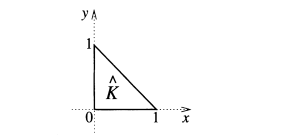
\includegraphics[width=0.33\textwidth]{referenzzelle.png} \\
	Abbildung aus \cite{knabner2013numerik} Seite 51
\end{figure}

\begin{Bemerkung}
	$\forall i,j\in\{1,2,3\}: \int_{F_j} \hat{\psi}_i \cdot \hat{n} \da = \delta_{i,j} \text{ und } \hat{\psi}_i \in \mathbb{P}_1(\hat{K}, \R^2).$
\end{Bemerkung}

Weiter setzen wir noch 
\begin{align*}
\text{ die Menge der Seiten }&& \hat{\mathcal{F}} &\coloneqq \left\{ \hat{F}_0, \hat{F}_1, \hat{F}_2 \right\} \\
\text{und den Seitenansatzraum }&&  \hat{W} &\coloneqq \spann \left\{ \psi_0,\psi_1, \psi_2 \right\}.
\end{align*}
\textbf{Transformation von $ \hat{K} $ zu $ K $:} Für ein beliebiges $ K \in \mathcal{K} $ wollen wir jetzt eine Seitenbasis $ \{ \psi_1^K, \psi_2^K, \psi_3^K \} $ berechnen (Wie bisher gegeben durch $ \forall i\in\{1,2,3\}: \psi_i^K\in\mathbb{P}_1(K,\R^2) \text{ und } \int_{F_j^K} \psi_i^K \cdot n^K \da = \delta_{i,j} $, wobei $ n^K $ äußere Normale von  $ K $ und $ F_j^K  $ beliebige Seite von $ K $). Dazu betrachten wir die affine Transformationsabbildung $ \varphi_K $ von $ \hat{K} $ zu $ K $:
\begin{align*}
\varphi_K: \hat{K} \to K, \varphi_K(\xi) = z_{0,K} + B_K \xi \text{ mit passenden } B_K\in\R^{2 \times 2} \text{ und } \\
J_K \coloneqq \det(B_K) > 0.
\end{align*}

\begin{figure}[H]
	\centering
	\captionabove{Affine lineare Transformation von $\hat{K}$ nach $ K $}
	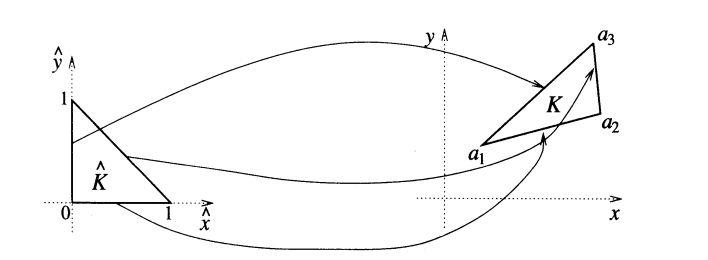
\includegraphics[width=0.55\textwidth]{affinlinearetransf.png} \\
	Abbildung aus \cite{knabner2013numerik} Seite 53
\end{figure} 

\begin{Lemma}
	Es gilt: $\tilde{n}^K = \frac{1}{\abs{B_K^{-T} \hat{n}}} B_K^{-T} \hat{n} $ ist Normale zu $ \partial K $.
\end{Lemma}

Die Seitenbasis auf $ K $ ist dann gegeben durch 
\[ \psi_i^K = J_K^{-1}B_K \hat{\psi}_i \circ \varphi_K \ (i\in \{1,2,3\}) \]

Die globale Seitenbasis $\{\psi_j\}_{j = 1}^{\abs{\mathcal{F}}}$ auf $ \mathbb{D}  $ erhalten wir dann mithilfe einer weiteren Abbildung $l$ die zwischen der Seitennummerierung in einer Zelle $ K $ und der globalen Seitennummerierung vermittelt. Es ist dabei
\[ l:\mathcal{K}\times \{1,2,3\} \to \{1, \dots , \abs{\mathcal{F}} \}, (K,i) \mapsto l(K,i). \]
Wir setzen nun also $ \psi_j (j \in \{1,\dots , \abs{\mathcal{F}}\})$ durch
\[ \psi_j(x) = 
\begin{cases}
\psi_i^K(x) , &\text{falls } j = l(K,i)\\
0,			  &\text{sonst}.
\end{cases} \]
\begin{Bemerkung}
	Für alle Zellen $ K \in \mathcal{K} $ von denen $ F_j $ eine anliegende Seite ($ \overline{K} \cap F_j \ne \emptyset $) und $ F_j $ lokal mit $ i \in \{1,2,3\} $ nummeriert ist, gilt:
	\[ \psi_j|_K = \psi_i^K. \]
\end{Bemerkung}

\subsubsection{Hybridisierung}

Wir betrachten die Räume
\[W_K \coloneqq \left\{ \psi_K:K \to \R^2: \psi_K = J_K^{-1}  B_K \hat{\psi} \circ \varphi_K^{-1}, \hat{\psi} \in \hat{W} \right\} \]
\[ W_\mathcal{K} \coloneqq \prod_{K \in \mathcal{K}} W_K, \qquad M_h \coloneqq \prod_{F \in \mathcal{F}} \mathbb{P}_0(F) \]
\[ M_h(u_D) \coloneqq \left\{ \mu_h \in M_h:\forall  F \subset \Gamma_D \int_F \mu_h \da = \int_F u_D \da  \right\}\]

\begin{Bemerkung}~
	
	$ \psi_h \in W_h \iff \big[ \psi_h \in W_{\mathcal{K}} \text{ und }  (\psi_{K_1} - \psi_{K_2}) \cdot n^F = 0 \ (F= \partial K_1 \cap \partial K_2 \in \mathcal{F}^{\circ})\big] $
\end{Bemerkung}


Und untersuchen folgendes Problem:
\begin{align*}
\text{Bestimmme } (q_h,u_h, \lambda_h) \in W_\mathcal{K} \times Q_h \times M_h(u_D) \text{ mit}\\
\begin{dcases}
(1) \int_K \kappa^{-1} q_h \psi_K \dx - \int_K u_h \dive(\psi_K) \dx = - \int_{\partial K} \lambda_h \psi_K \cdot n^K \da \\
(2) \int_K \dive(q_h) \phi_K \dx = 0\\
(3) \sum_{K\in \mathcal{K}} \int_{\partial K} q_h \cdot n \mu_h \da = - \int_{\Gamma_N} g_N \mu_h \da
\end{dcases}\\
\text{für alle } K \in \mathcal{K}, \psi_K \in W_K, \phi_K \in Q_h  \text{ und } \mu_h \in M_h(0)
\end{align*}

Dieses Problem ist äquivalent zu dem diskreten gemischten FE-Problem, welches wir zuvor betrachtet haben:
\begin{align*}
\text{Bestimme } (q_h,u_h) \in W_h(-g_N) \times Q_h \text{ mit}\\
\begin{cases}
\int_{\Omega} \kappa ^{-1} q_h \cdot \psi_h \dx \mkern-15mu &- \int_{\Omega} u_h \dive(\psi_h) \dx = - \int_{\Gamma_D} u_D \psi_h \cdot n \da\\
&- \int_{\Omega} \dive(q_h) \phi_h \dx = 0
\end{cases} \\
\text{für alle } (\psi_h, \phi_h) \in W_h(0) \times Q_h
\end{align*}

Für ein festes $ K \in \mathcal{K} $ ergibt sich mit der Wahl einer Basis von $ W_K $, $ Q_h $ und $ M_h $ 
%\begin{align*}
%	&W_K = \spann\{\psi_F \mid F \in \mathcal{F}_K \}  &&(\psi_F \cdot n^F)_{|F'} = \begin{cases}
%		1 &F = F'\\
%		0 &\text{sonst}
%	\end{cases}\\
%	&Q_h = \spann\{\eta_K \mid K \in \mathcal{K}  \}  &&{\eta_K}_{|K'} = \begin{cases}
%	1 &, K = K'\\
%	0 &,\text{sonst}
%	\end{cases}\\
%	&M_h = \spann \{ \nu_F \mid F \in \mathcal{F}_K \}  &&{\nu_F}_{|F'} = \begin{cases}
%		1 &, F = F'\\
%		0 &, \text{sonst}
%	\end{cases}  
%\end{align*}

eine Formulierung als LGS mit Nebenbedingung, wobei $ \ubar{q}_K \coloneqq \ubar{R}_K \ubar{q}, \ \ubar{u}_K \coloneqq \ubar{R}_K \ubar{u} $
\begin{align*}
\text{Bestimme } \ubar{q}, \ubar{u} \text{ und } \ubar{\lambda} \text{ mit}\\
\begin{dcases}
(1) \begin{pmatrix}
\ubar{A}_K & \ubar{B}_K \\
\ubar{B}_K^T & 0
\end{pmatrix}
\begin{pmatrix}
\ubar{q}_K\\
\ubar{u}_K
\end{pmatrix}
\mkern-16mu&= \begin{pmatrix}
- \ubar{C}_K \, \ubar{R}_K \ubar{\lambda} \\
0
\end{pmatrix}\\
(2) \sum_{K \in \mathcal{K}}  (\ubar{R}_K \ubar{\mu})^T \ubar{C}_K \ubar{q}_K \mkern-16mu&= \ubar{\mu}^T \ubar{b}		
\end{dcases}\\
\text{für alle } \ubar{\mu} \text{ mit } \ubar{\mu}[F] = 0 \text{ für } F \in \Gamma_D \cap \mathcal{F}
\end{align*}

\begin{align*}
\left(
\begin{array}{c}
1\\ 1 \\ \vdots \\ 1 \\ 1\\ \ubar{\mu}
\end{array}
\right)^T
\underbrace{\left(
	\begin{array}{ccccc|c}
	\ubar{A}_{K_1} & \ubar{B}_{K_1}&&&& \ubar{C}_{K_1} \ubar{R}_{K_1}\\
	\ubar{B}_{K_1} & 0 &&&& 0\\
	&& \ubar{A}_{K_2} & \ubar{B}_{K_2} && \ubar{C}_{K_2} \ubar{R}_{K_2}\\
	&  & \ubar{B}_{K_2} & 0 && 0\\
	&  &  &  &\ddots &\\
	\hline
	\ubar{R}_{K_1}^T \ubar{C}_{K_1}^T& 0 & \ubar{R}_{K_2}^T \ubar{C}_{K_2}^T& 0& &0 \\
	\end{array}
	\right)}_{\eqqcolon \left( \begin{array}{c|c}
	\ubar{D} & \ubar{E}\\
	\hline
	\ubar{E}^T & 0
	\end{array} \right)}
\underbrace{\left(
	\begin{array}{c}
	\ubar{q}_{K_1}\\ \ubar{u}_{K_1} \\ \ubar{q}_{K_2}\\ \ubar{u}_{K_2} \\ \vdots \\ \ubar{\lambda}
	\end{array}
	\right)}_{\eqqcolon \left( \begin{array}{c}
	\left(
	\begin{array}{c}
	\ubar{q}_{K_i}\\ \ubar{u}_{K_i}
	\end{array}
	\right)_{K_i \in \mathcal{K}} \\ \ubar{\lambda} 
	\end{array}\right)} = 
\left(
\begin{array}{c}
0\\ 0 \\ \vdots \\ 0 \\ 0\\ \ubar{\mu}^T \ubar{b}
\end{array}
\right)
\end{align*}
Mit dem Schurkomplement $ \ubar{S} \coloneqq \ubar{E}^T \ubar{D}^{-1} \ubar{E} $ folgt
\[ \ubar{\mu}^T \ubar{S} \, \ubar{\lambda} = \ubar{\mu}^T \ubar{b} 	\text{ für alle } \ubar{\mu} \text{ mit } \ubar{\mu}[F] = 0 \text{ für } F \in \Gamma_D \cap \mathcal{F} \]

Sobald wir $ \ubar{\lambda}_k \coloneqq \ubar{R}_K \ubar{\lambda}$ bestimmt haben, können wir auch das obere LGS (1) lösen um $ \ubar{q}_K $ und $ \ubar{u}_K $ zu erhalten.
% Um $ \ubar{\lambda}_k $ zu erhalten lösen wir das globales System:
%\begin{align*}
%	\underline{S} \, \underline{\lambda} = \underline{b}
%\end{align*}
%und bekommen somit $ \ubar{\lambda}_k $ über die Restriktionen
%\[ \ubar{\lambda} = \sum_{K \in \mathcal{K}} \ubar{R}_K \ubar{\lambda}_K .\]







